\section{Perancangan Akselerator Perangkat Keras}
\label{sec:perancangan-akselerator}

Implementasi akselerator perangkat keras yang lengkap, sampai dapat digunakan pada tingkatan perangkat lunak, memerlukan dua komponen penting untuk dibangun sebagai berikut.

\begin{enumerate}
	\item Implementasi ekstensi instruksi RISC-V di \textit{processor} VeeR EL2.
	\item \ac{BSP} untuk akses ekstensi RISC-V pada perangkat lunak.
\end{enumerate}

Kedua komponen tersebut, kemudian perlu diuji akurasinya menggunakan perangkat lunak \textit{verilator} \parencite{verilator2024github}. Desain dan implementasi dari kedua komponen beserta pengaturan pengujiannya akan dijelaskan pada sub sub-bab selanjutnya.

\subsection{Implementasi Ekstensi Instruksi RISC-V di \textit{Processor} VeeR EL2}

Agar dapat membangun akselerator perangkat keras yang dapat digunakan secara \textit{generic}, maka perlu dibuat sebuah separasi jelas bagian komputasi yang ingin dioptimasi menggunakan perangkat keras dan bagian yang tetap berada pada tingkat perangkat lunak agar dapat dibuat secara fleksibel oleh pendesain agen \ac{RL}. Pembagian ini, umumnya disebut sebagai \textit{hardware/software} (HW/SW) \textit{co-design}. Pada kasus pengembangan akselerator perangkat keras ini, HW/SW \textit{co-design} dilakukan sesuai dengan deskripsi pada Algoritma \ref{alg:hw-sw-sep}.

\begin{algorithm}
	\makeatletter
	\renewcommand{\ALG@name}{Algoritma}
	\makeatother
	\caption{Pembagian HW/SW \textit{co-design}}\label{alg:hw-sw-sep}
	\renewcommand{\algorithmicrequire}{\textbf{Masukan:}}
	\renewcommand{\algorithmicensure}{\textbf{Keluaran:}}
	\begin{algorithmic}[1]
		\Require jumlah episode, \textit{learning rate} ($\alpha$), dan \textit{discount factor} ($\gamma$)
		\Ensure \textit{Q-Table}
		\State \alghighlight{yellow!50}{Inisialisasi \textit{Q-Table} untuk setiap \textit{state} dan aksi \label{algline:initialize-q-table-hw} \Comment{\textbf{Perangkat keras}}}
		\State \alghighlight{yellow!50}{Simpan $\gamma$ dan $\alpha$ pada akselerator \Comment{\textbf{Perangkat keras}}}
		\While{$banyak\_episode < jumlah\_episode$}
		\State $s_{t} \gets s_0$
		\While{$s_t \neq s_{terminal}$}
		\State \alghighlight{yellow!50}{Pilih aksi ($A$) untuk \textit{state} kini ($s_t$) \label{algline:choose-action-hw}  \Comment{\textbf{Perangkat keras}}}
		\State Lakukan $A$, dapatkan \textit{reward} dan $s_{t+1}$
		\State \alghighlight{yellow!50}{Simpan $s_{t+1}$ pada akselerator \Comment{\textbf{Perangkat keras}}}
		\State \alghighlight{yellow!50}{Hitung nilai \textit{Q-Table} indeks terkini \label{algline:q-table-update-hw} \Comment{\textbf{Perangkat keras}}}
		\State $s_t \gets s_{t+1}$
		\EndWhile
		\State $banyak\_episode \gets banyak\_episode + 1$
		\State $cr_t$ $\gets$ \textit{cumulative reward} dari \textit{Q-Table}
		\If{$cr_t\ >\ cr_{t-1}$}
		\State Ubah nilai $maxQ(s_{t+1},a))$ dari \textit{Q-Table}
		\EndIf
		\State $cr_{t-1} \gets cr_t$
		\State \textit{memori Q-Table} $\gets$ \textit{Q-Table}
		\State $episode \gets episode + 1$
		\EndWhile
	\end{algorithmic}
\end{algorithm}

Baris pada Algoritma \ref{alg:hw-sw-sep} yang berwarna kuning dan berkomentar "Perangkat Keras" merupakan bagian dari Algoritma \ref{alg:rl-qmemo} yang dioptimasi menggunakan akselerator perangkat keras. Implementasi dari perangkat keras tersebut berupa ekstensi modul pada \textit{processor} VeeR EL2 yang memiliki detail implementasi sesuai pada ilustrasi di Lampiran \ref{appendix:veer-el2-full}. Pada ilustrasi tersebut, terdapat sebuah fitur \textit{out-of-pipe divider} pada \textit{decode stage} dari \textit{processor} VeeR EL2 pada Gambar \ref{fig:veer-el2-decode}.

\begin{figure}[H]
	\centering
	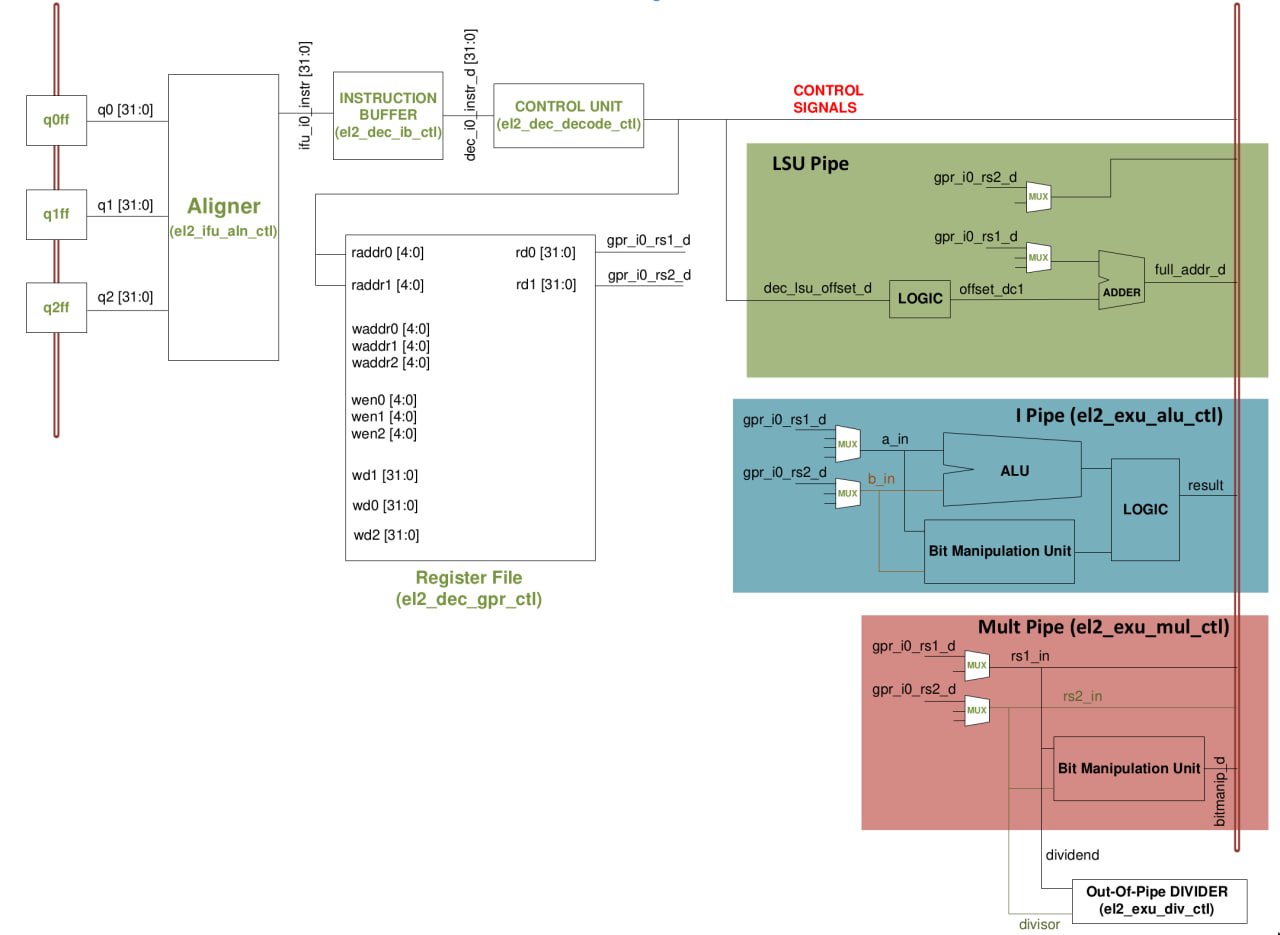
\includegraphics[width=1\textwidth]{chapter-3/veer-el2-decode.jpg}
	\caption{\textit{Processor} VeeR EL2 pada \textit{Decode Stage}}
	\label{fig:veer-el2-decode}
\end{figure}

Pada \textit{decode stage}, instruksi akan diteruskan kepada \textit{execute} dan \textit{memory stage} untuk akhirnya dieksekusi sesuai dengan jenis instruksi. Pada \textit{execute} dan \textit{memory stage}, terdapat tiga jenis kemungkinan operasi sebagai berikut.


\begin{enumerate}
	\item \ac{LSU}: merupakan unit eksekusi yang berurusan dengan keperluan akses baca dan menulis memori pada \ac{RAM}.
	\item \textit{Integer} \ac{ALU}: merupakan unit eksekusi yang berurusan dengan operasi tambah dan kurang untuk tipe \textit{integer}. Unit ini juga digunakan untuk keperluan menghitung \textit{offset} dari alamat memori bila diperlukan. Selain itu, unit ini, karena sering digunakan, diduplikat menjadi dua unit agar dapat digunakan secara paralel.
	\item \textit{Multiplier Unit}: merupakan unit yang digunakan untuk melakukan operasi pengalian untuk tipe \textit{integer}.
\end{enumerate}

Selain tiga unit eksekusi diatas, terdapat sebuah unit \textit{out-of-pipe divider} yang merupakan unit untuk melakukan operasi pembagian tipe \textit{integer}. Perbedaan yang dimiliki oleh unit \textit{out-of-pipe divider} adalah unit ini tidak terhubung dengan jalur \textit{pipelining} yang sama dengan unit lain, sehingga dapat mengimplementasikan logika pada \textit{writeback stage} secara mandiri. Selain itu, karena unit ini tidak terhubung dengan jalur \textit{pipelining} unit lain, maka unit ini dapat digunakan sebagai tempat implementasi ekstensi untuk akselerator perangkat keras. Pada Gambar \ref{fig:out-of-pipe}, diilustrasikan diagram blok logika yang digunakan untuk implementasi akselerator perangkat keras \ac{RL} yang berada pada unit \textit{out-of-pipe divider}.

\begin{figure}[H]
	\centering
	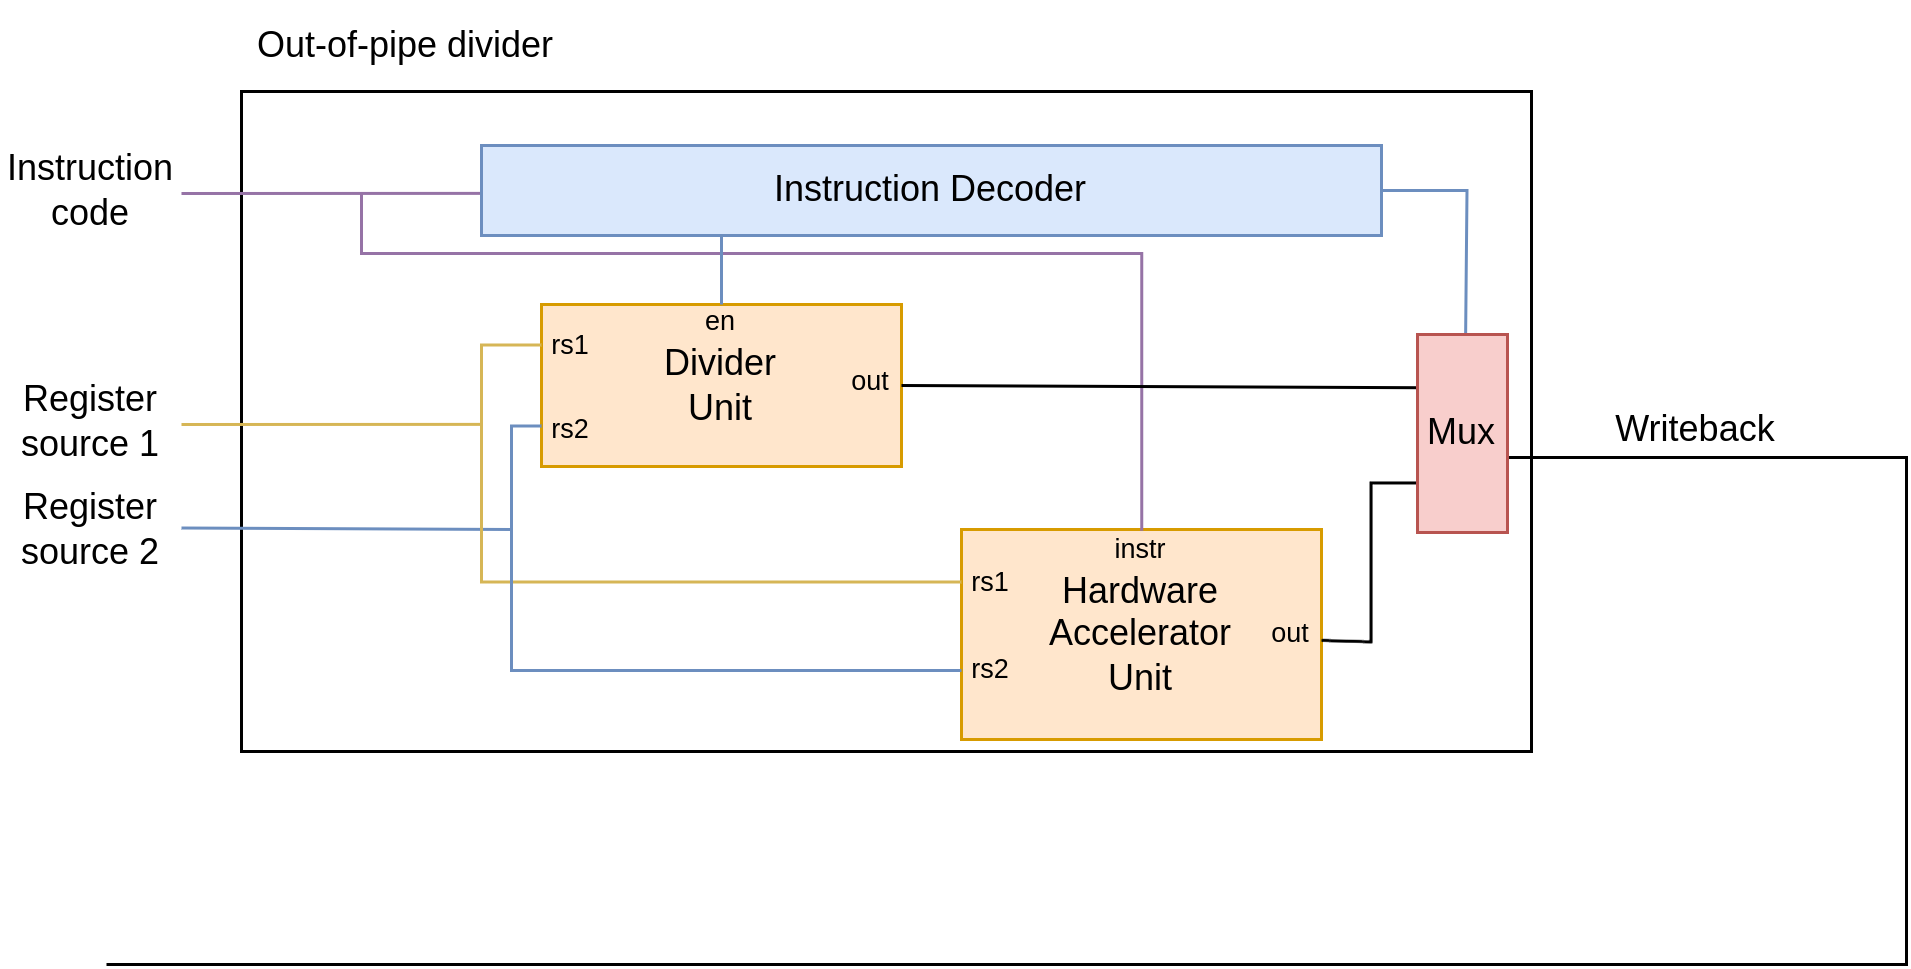
\includegraphics[width=1\textwidth]{chapter-3/out-of-pipe.png}
	\caption{Unit \textit{Out-of-pipe} \textit{Decode Stage}}
	\label{fig:out-of-pipe}
\end{figure}

Unit \textit{out-of-pipe}, seperti tergambar di Gambar \ref{fig:out-of-pipe}, diubah agar tidak hanya berisikan unit \textit{divider integer} tapi juga akselerator perangkat keras untuk \ac{RL}. Implementasi akselerator pada unit \textit{out-of-pipe} memiliki keuntungan terhindarnya ekstensi instruksi dari \textit{hazard}. \textit{Hazard} merupakan sebuah kondisi pada \textit{pipelined processor}, dimana perhitungan secara paralel mengalami kesalahan karena ketidaksesuaian urutan dari penyelesaian instruksi \parencite{sarah2021digital}.

Implementasi akselerator perangkat lunak memiliki empat komponen utama sebagai berikut.

\begin{enumerate}
	\item \textit{Q-Table \ac{LSU}}\\
	      Merupakan sebuah unit yang berfungsi sebagai pengganti dari penyimpanan \textit{Q-Table} pada perangkat lunak. Pada perangkat lunak, representasi \textit{Q-Table} dapat merupakan sebuah data struktur seperti \textit{array, hashmap}, dan \textit{linked list}. Pengganti data struktur tersebut pada akselerator perangkat keras ini adalah blok \ac{RAM}.
	\item \textit{Constant Registers}\\
	      Merupakan kumpulan dari \textit{register} yang digunakan untuk menyimpan tiga nilai pada Persamaan \ref{eq:q-learning}: $\alpha$, $gamma$, dan $s_t$. \textit{Register} merupakan kumpulan dari flip flop dengan \textit{common clock} yang merepresentasikan sekumpulan bit informasi \parencite{sarah2021digital}.
	\item \textit{Q-Table Updater}\\
	      Merupakan sebuah unit utama yang melakukan komputasi Persamaan \ref{eq:q-learning}.
	\item \textit{Max Seeker Unit}\\
	      Merupakan unit yang dapat menghasilkan dua nilai: $maxQ(s_{t+1},a)$ dan $a_{max}$, aksi yang menghasilkan $maxQ(s_{t+1},a)$.
\end{enumerate}


Secara lebih detail, implementasi dari seluruh komponen unit tersebut secara lengkap pada akselerator diilustrasikan pada Gambar \ref{fig:hw-accel}.

\begin{figure}[H]
	\centering
	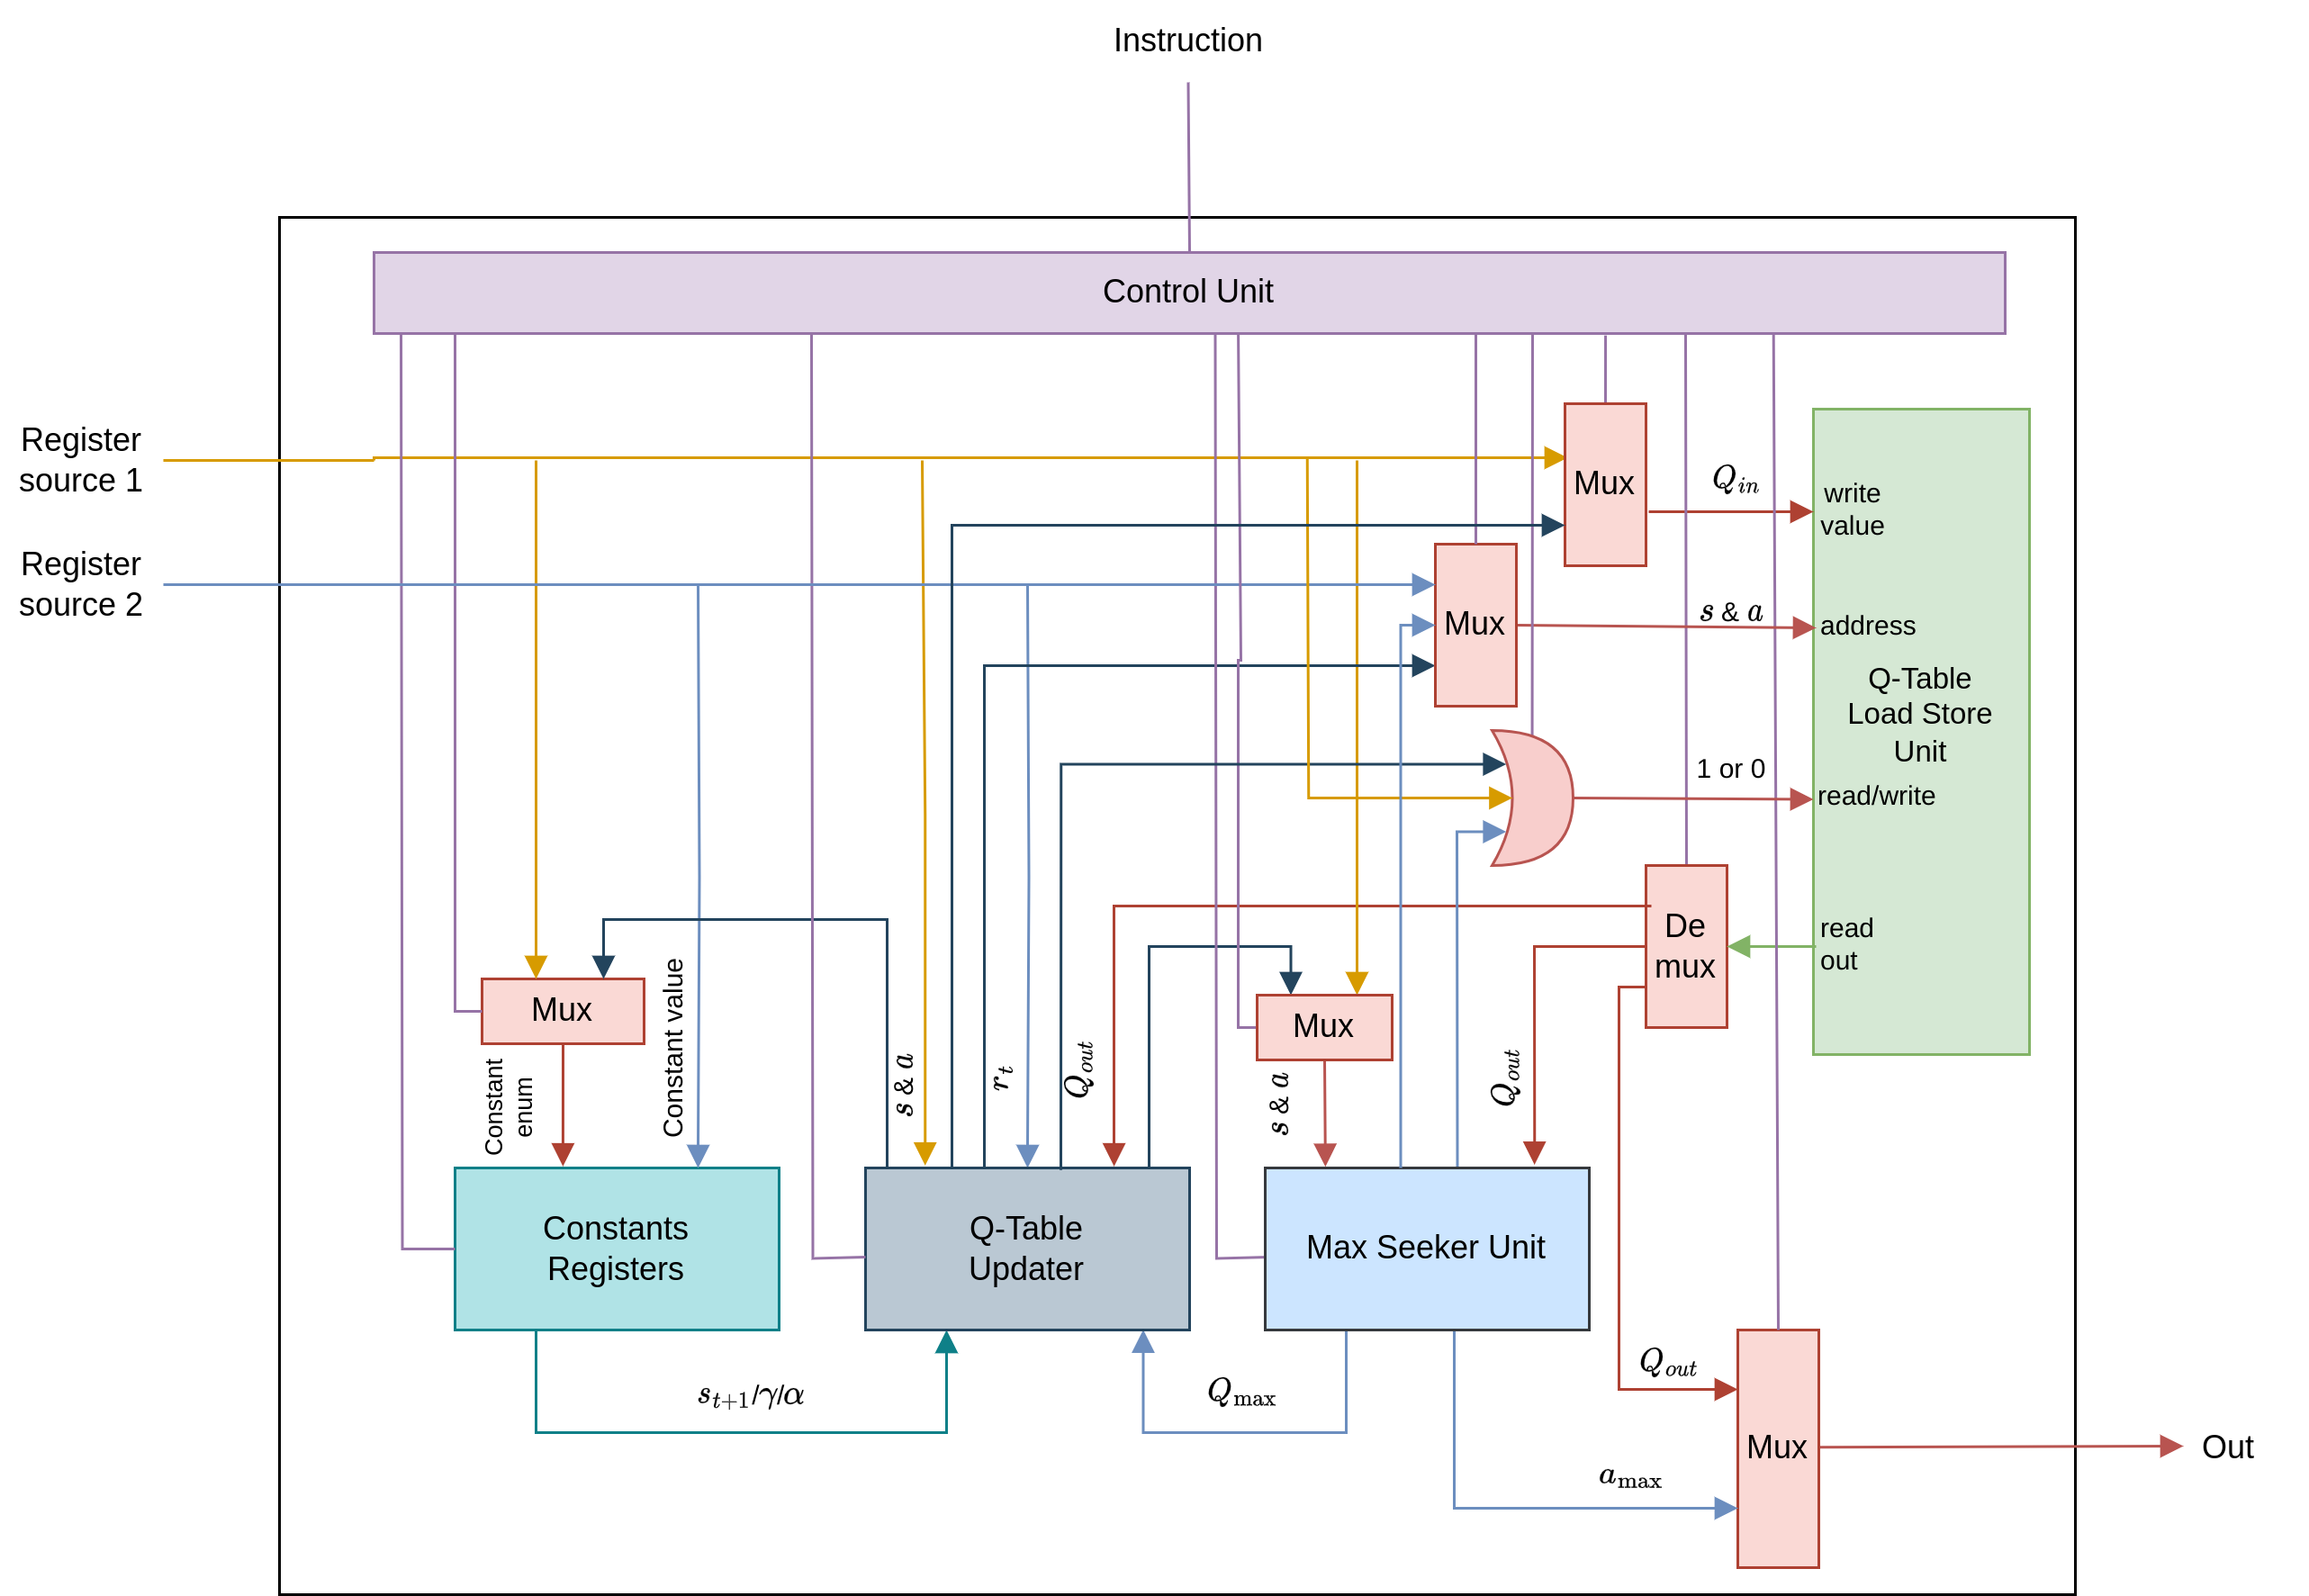
\includegraphics[width=1\textwidth]{chapter-3/hw-accel.png}
	\caption{Unit Akselerator Perangkat Keras}
	\label{fig:hw-accel}
\end{figure}

Komponen-komponen pada akselerator, sesuai pada Gambar \ref{fig:hw-accel}, digunakan untuk mengimplementasikan lima ekstensi instruksi sebagai berikut.

\begin{enumerate}
	\item q.store\\
	      Merupakan instruksi yang digunakan untuk menyimpan sebuah nilai pada \textit{Q-Table} dari perangkat lunak ke \textit{Q-Table \ac{LSU}}.
	\item q.load\\
	      Merupakan instruksi yang digunakan untuk mendapatkan sebuah nilai dari \textit{Q-Table \ac{LSU}} ke perangkat lunak.
	\item q.max\\
	      Merupakan instruksi yang digunakan untuk mendapatkan nilai $a_{max}$ dari \textit{Max Seeker Unit} ke perangkat lunak.
	\item q.store\_constant\\
	      Merupakan instruksi yang digunakan untuk menyimpan nilai $\alpha$, $\gamma$ dan $s_{t+1}$ dari perangkat lunak ke \textit{Constant Registers}.
	\item q.update\\
	      Merupakan instruksi yang digunakan untuk memberikan nilai $r$, $s_t$, dan $a_t$ dan menyimpan hasil perhitungan dari Persamaan \ref{eq:q-learning} oleh \textit{Q-Table Updater} ke \textit{Q-Table \ac{LSU}}.
\end{enumerate}

Secara berurutan, mengacu kepada Algoritma \ref{alg:hw-sw-sep}, penggunaan akselerator akan dimulai pada baris \ref{algline:initialize-q-table-hw} dengan inisiasi \textit{Q-Table} menggunakan instruksi q.load untuk menyimpan nilai kepada \textit{Q-Table \ac{LSU}}. Secara detail, Gambar \ref{fig:q-table-lsu} merupakan ilustrasi dari \textit{Q-Table \ac{LSU}} yang digunakan untuk menyimpan nilai \textit{Q-Table}.

\begin{figure}[H]
	\centering
	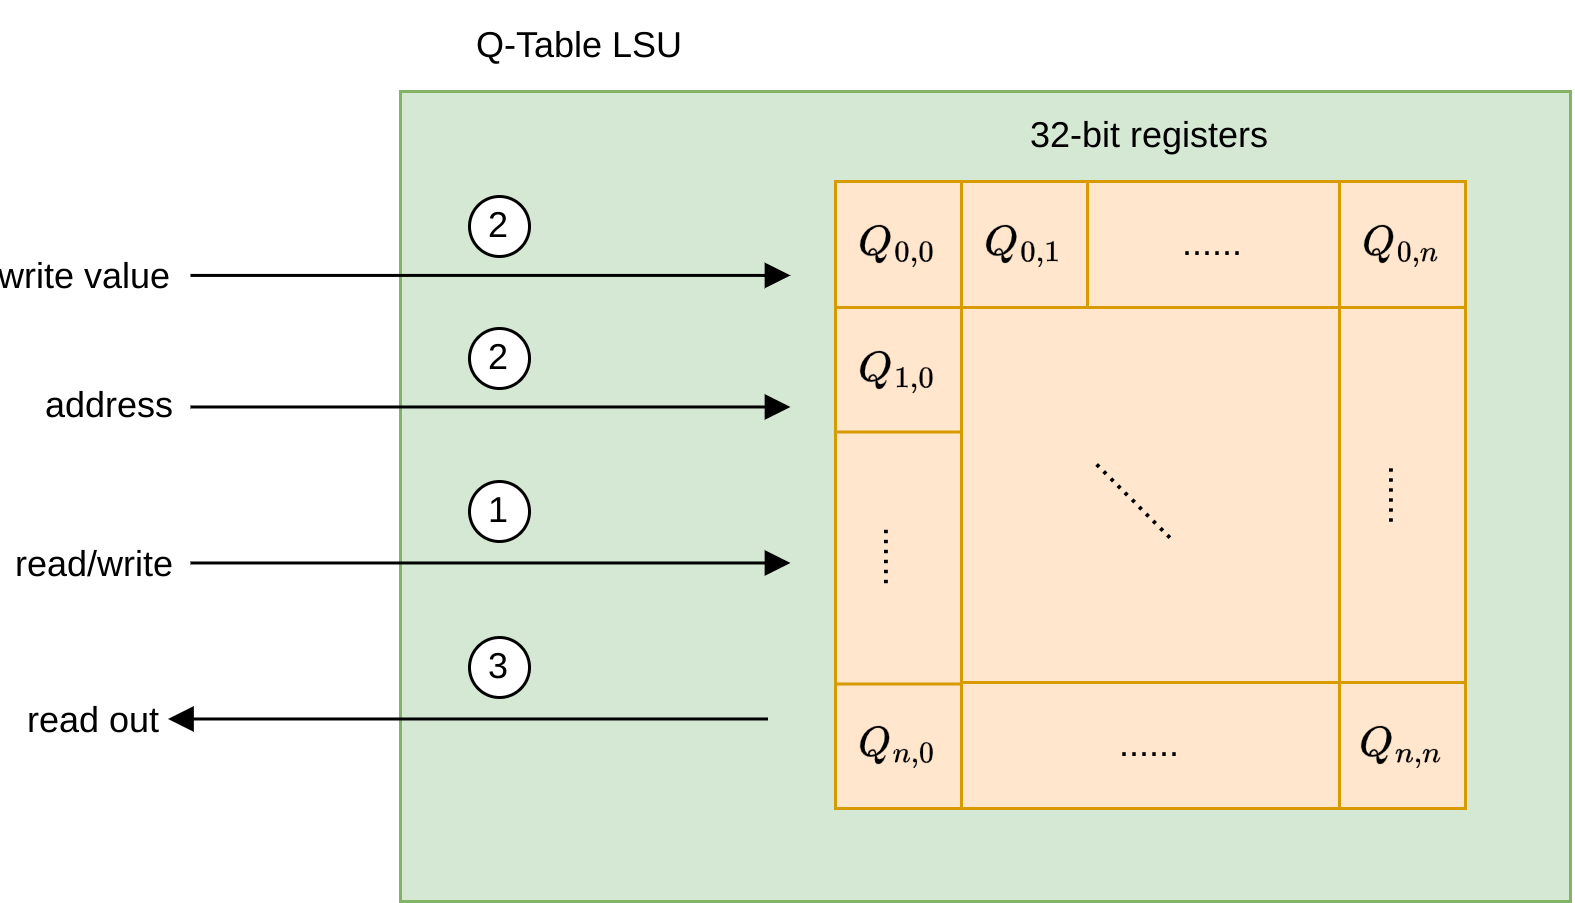
\includegraphics[width=1\textwidth]{chapter-3/q-table-lsu.png}
	\caption{Ilustrasi Penggunaan \textit{Q-Table LSU}}
	\label{fig:q-table-lsu}
\end{figure}

Gambar \ref{fig:q-table-lsu}, memberikan detail dari tahapan penulisan kepada blok \ac{RAM} untuk \textit{Q-Table} menggunakan \textit{Q-Table \ac{LSU}}. Pertama, input \textit{read/write} berupa biner 1-bit akan digunakan untuk menentukan operasi yang dilakukan antara penulisan atau pembacaan nilai pada \ac{RAM}. Kedua, input \textit{address} digunakan untuk menentukan nilai \textit{Q-Table} mana yang akan ditulis/dibaca. \textit{address} yang digunakan pada kasus dihitung dari $s_t \times N_a + a_t$ dengan $N_a$ sebagai banyaknya aksi yang digunakan pada konteks lingkungan \ac{RL}. Pada saat yang bersamaan dengan pembacaan input \textit{address}, dilakukan pembacaan input \textit{write value} untuk menuliskan nilai ke blok \ac{RAM} \textit{Q-Table} apabila pembacaan input \textit{read/write} menyatakan \textit{write}. Terakhir, apabila pembacaan \textit{read/write} menyatakan \textit{read} maka akan nilai dari \textit{register} dengan alamat sesuai dengan input \textit{address} akan diberikan kepada keluaran \textit{read out}.

Lalu, setelah dilakukannya inisiasi \textit{Q-Table} pada baris \ref{algline:initialize-q-table-hw}, program akan dilanjutkan untuk menyimpan nilai konstanta $\alpha$ dan $\gamma$ untuk perhitungan Persamaan \ref{eq:q-learning} pada baris \ref{algline:q-memo-equation}. Penyimpanan nilai konstanta akan dilakukan menggunakan instruksi q.store\_constant, nilai konstanta tersebut akan disimpan pada unit \textit{Constant Registers} yang memiliki fungsionalitas yang sama dengan \textit{Q-Table \ac{LSU}} yaitu untuk menyimpan data ke \textit{register} internal dari akselerator. Arsitektur dari \textit{Constant Registers} tergambar pada Gambar \ref{fig:constant-registers}.

\begin{figure}[H]
	\centering
	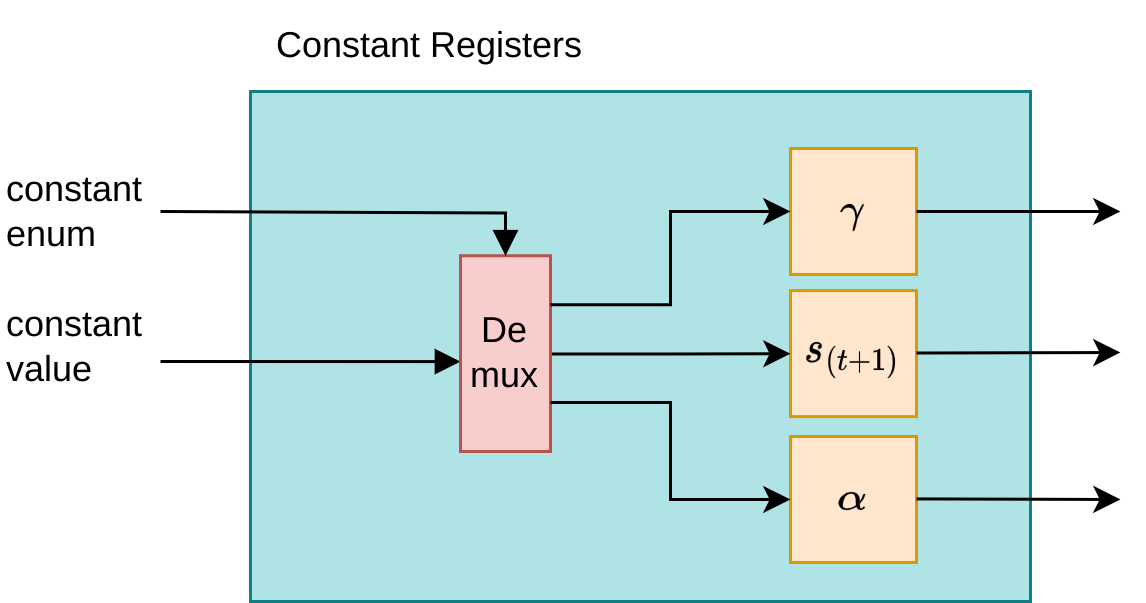
\includegraphics[width=1\textwidth]{chapter-3/constant-registers.png}
	\caption{Ilustrasi Penggunaan \textit{Constant Registers}}
	\label{fig:constant-registers}
\end{figure}

\textit{Constant Registers} pada Gambar \ref{fig:constant-registers} memiliki input \textit{constant value} dan \textit{constant enum}. \textit{Constant value} merupakan nilai dari konstanta yang akan disimpan, sedangkan \textit{constant enum} merupakan nilai yang akan menentukan kepada \textit{register} mana \textit{constant value} akan disimpan.

Lalu, setelah penyimpanan nilai konstanta $\alpha$ dan $\gamma$, penggunaan akselerator perangkat keras dilanjutkan pada baris \ref{algline:choose-action-hw} untuk memilih aksi yang digunakan untuk pembelajaran agen \ac{RL}. Pemilihan aksi pada penelitian ini dilakukan penggunakan pendekatan \textit{$\epsilon$-greedy} \parencite{christopher1989learning}. Pendekatan \textit{$\epsilon$-greedy} berarti membagi pemilihan aksi menjadi dua kemungkinan sebagai berikut.

\begin{enumerate}
	\item Eksplorasi\\
	      Merupakan sebuah pemilihan aksi secara acak. Pemilihan acak ini dilakukan agar agen \ac{RL} dapat mempelajari sebuah posibilitas pemilihan aksi yang sebelumnya belum dianggap sebagai aksi terbaik.
	\item Eksploitasi\\
	      Merupakan sebuah pemilihan aksi terbaik berdasarkan nilai yang ada pada \textit{Q-Table}. Pada penelitian ini, desain fungsi \textit{reward} sesuai dengan \ref{algline:q-reward}, memberikan nilai yang besar untuk indikasi sebuah aksi yang baik diambil. Sehingga, eksploitasi dilakukan dengan memilih aksi yang memberikan nilai \textit{Q-Table} terbesar ($a_{max}$).
\end{enumerate}

Kedua pemilihan aksi tersebut, ditentukan secara acak dengan pembagian probabilitas yang diatur oleh konstanta $\epsilon$. Bagian yang optimasi menggunakan akselerator perangkat keras adalah pemilihan aksi menggunakan metode eksploitasi. Bagian dari unit akselerator yang digunakan untuk melakukan metode eksploitasi tersebut adalah \textit{Max Seeker Unit}. Nilai $a_{max}$ akan didapatkan dari \textit{Max Seeker Unit} menggunakan ekstensi instruksi q.max. Secara detail, Gambar \ref{fig:max-seeker-unit} merupakan ilustrasi detail dari \textit{Max Seeker Unit}.

\begin{figure}[H]
	\centering
	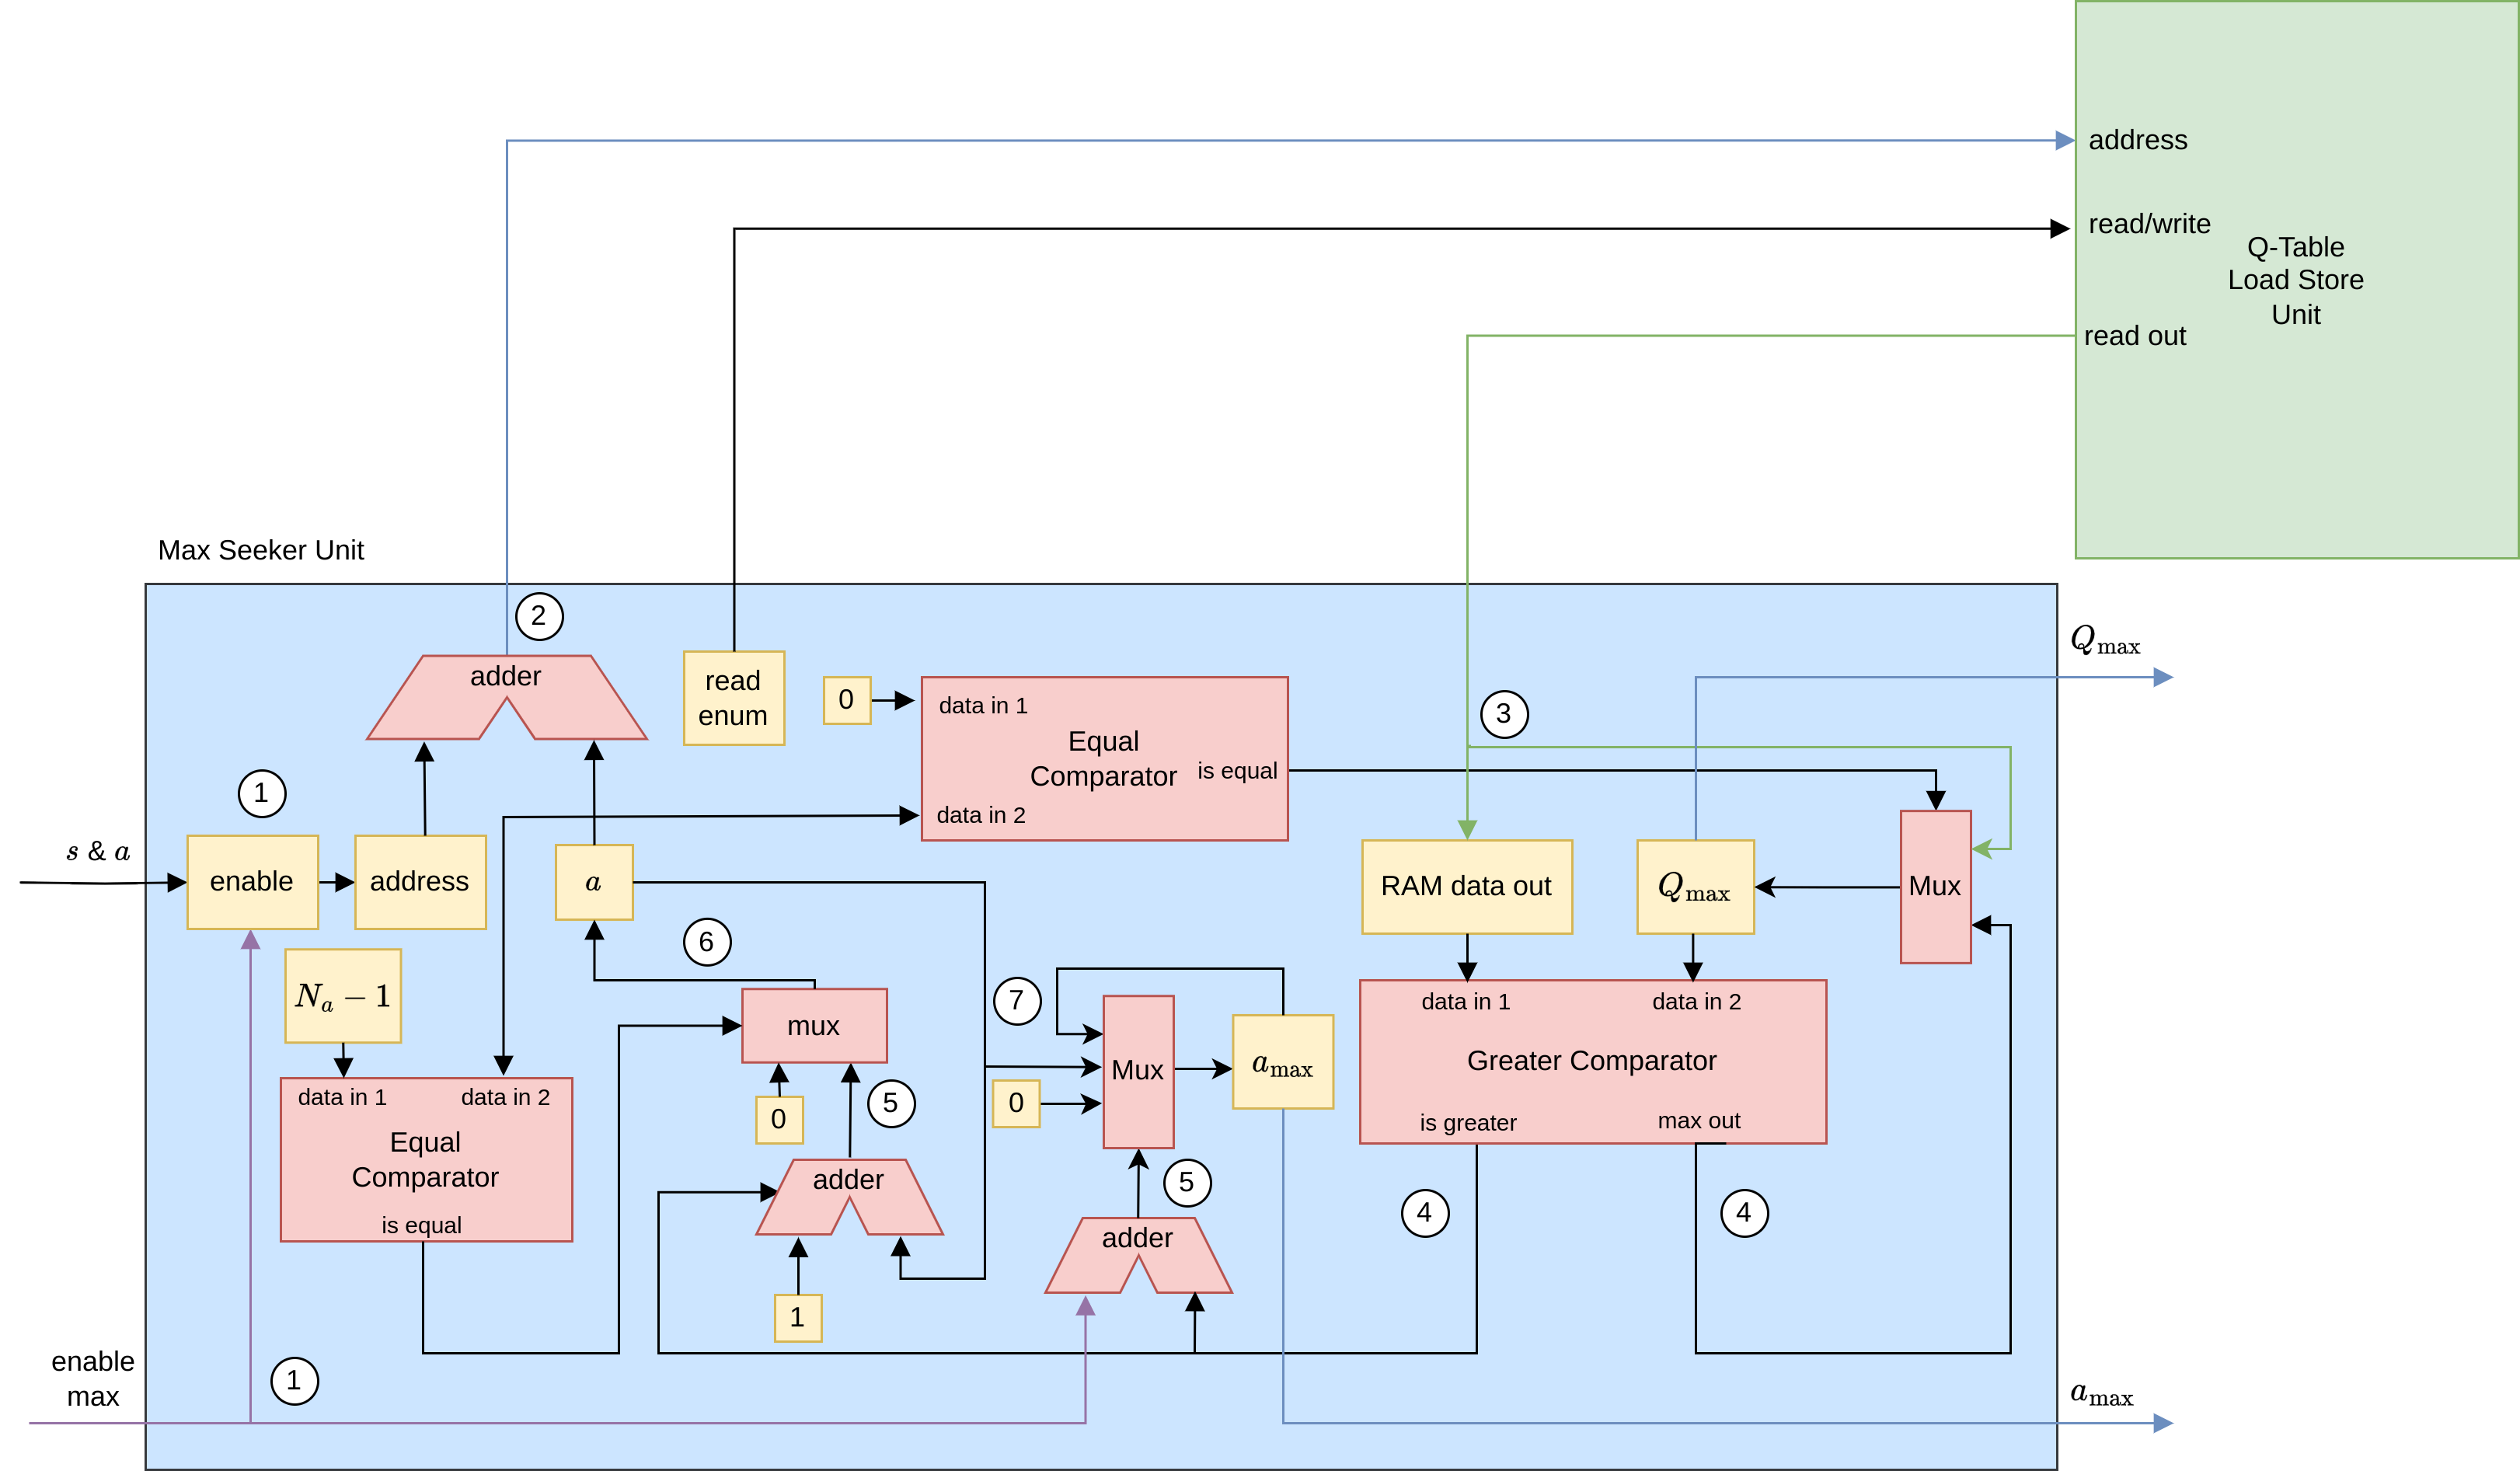
\includegraphics[width=1\textwidth]{chapter-3/max-seeker-unit.png}
	\caption{Ilustrasi Penggunaan \textit{Max Seeker Unit}}
	\label{fig:max-seeker-unit}
\end{figure}

Pada Gambar \ref{fig:max-seeker-unit}, digambarkan tahapan-tahapan yang digunakan untuk mendapatkan nilai $a_{max}$ dari \textit{Max Seeker Unit} menggunakan instruksi q.max. Secara singkat, \textit{Max Seeker Unit} mengambil nilai \textit{Q-Table} dari alamat dasar, sampai alamat dasar ditambah $N_a$. Lalu, semua nilai \textit{Q-Table} tersebut dibandingkan dan disimpan nilai terbesar dan index dari nilai terbesar tersebut sebagai keluaran. Berikut merupakan penjelasan dari tahapan-tahapan tersebut secara berurutan.

\begin{enumerate}
	\item Pada tahap pertama, \textit{register source} 1 akan bernilai $s$ sebagai alamat dasar dari operasi pengambilan data dari \textit{Q-Table \ac{LSU}}. Pada saat bersamaan, masuk dari \textit{control unit} nilai \textit{enable max} yang mengatur mulainya operasi dari \textit{Max Seeker Unit}.
	\item Setelah \textit{enable max} masuk, $s$ dari \textit{register source} 1 akan ditambahkan dengan $a$. $a$ merupakan \textit{register} yang digunakan sebagai indeks yang digunakan untuk mencari $a_{max}$. Hasil dari penambahan $s$ dengan $a$ akan digunakan untuk mendapatkan nilai $Q_{(s,a)}$ dari \textit{Q-Table \ac{LSU}}.
	\item Nilai $Q_{(s,a)}$ didapatkan dari \textit{Q-Table \ac{LSU}}. Nilai ini akan digunakan untuk dilihat perbandingannya dengan \textit{register} $Q_{max}$. \textit{Register} $Q_{max}$ merupakan \textit{register} yang digunakan untuk menyimpan data $Q_{(s,a)}$ terbesar. Saat $a$ bernilai nol, maka nilai $Q_{(s,a)}$ akan disimpan langsung kepada $Q_{max}$. Penentuan nilai $a$ bernilai nol didapatkan dari hasil keluaran dari \textit{equal comparator}. Nilai keluarannya, kemudian digunakan oleh \ac{MUX} yang mendapatkan sinyal pemilihan nilai yang masuk untuk $Q_{max}$. \label{listline:max-seeker-start}
	\item Bila nilai $a$ tidak nol, maka nilai $Q_{max}$ akan bergantung kepada keluaran dari \textit{greater comparator}. Bila nilai hasil dari \textit{greater comparator} antara $Q_{max}$ dan keluaran dari \textit{Q-Table \ac{LSU}} adalah nilai \textit{Q-Table \ac{LSU}} yang lebih besar, maka sinyal keluaran \textit{is greater} akan menjadi \textit{HIGH} dan \textit{max out} akan mengeluarkan nilai tertinggi antara kedua nilai yang dikomparasi.
	\item Nilai keluaran dari \textit{is greater} akan digunakan untuk dua hal. Pertama, nilai \textit{is greater} akan digunakan untuk sinyal kontrol kepada \ac{MUX} yang digunakan untuk menentukan nilai masukan kepada $a_{max}$. Kedua, nilai \textit{is greater} akan digunakan sebagai sinyal kontrol untuk rangkaian \textit{adder} untuk memulai penambahan iterasi nilai \textit{register} $a$.
	\item Nilai keluaran dari rangkaian \textit{adder} yang dikontrol oleh keluaran \textit{is greater} akan digunakan untuk pembaruan nilai \textit{register} $a$.
	\item Nilai \textit{register} $a$ akan digunakan untuk membarui nilai \textit{register} $a_{max}$ berdasarkan tiga kondisi yang diatur oleh \ac{MUX}. Pertama, bila nilai \textit{enable max} \textit{HIGH} namun nilai \textit{is greater} tidak, maka nilai $a_{max}$ akan tetap seperti sebelumnya. Kedua, bila nilai \textit{enable max} dan \textit{is greater} bernilai \textit{HIGH}, maka nilai $a_{max}$ akan mengambil nilai dari $a$. Terakhir, bila kedua nilai \textit{enable max} dan \textit{is greater} bernilai \textit{LOW}, maka nilai $a_max$ akan mengambil nilai nol karena berarti modul belum dimulai. \label{listline:max-seeker-end}
\end{enumerate}

Langkah yang diambil dari nomor \ref{listline:max-seeker-start} hingga \ref{listline:max-seeker-end} akan diulang sampai $a$ bernilai $N_a - 1$. Setelah itu, nilai $Q_{max}$ dan $a_{max}$ akan menjadi keluaran dari \textit{Max Seeker Unit}. Setelah pemilihan nilai $a_{max}$ dilakukan dari \textit{Max Seeker Unit}, maka bagian algoritma selanjutnya yang menggunakan akselerator perangkat keras adalah pembaruan nilai \textit{Q-Table} menggunakan Persamaan \ref{eq:q-learning} pada baris \ref{algline:q-table-update-hw}. Pembaruan nilai \textit{Q-Table} dilakukan menggunakan unit \textit{Q-Table Updater} dengan instruksi q.update. Pada Gambar \ref{fig:q-table-updater}, dideskripsikan unit \textit{Q-Table Updater} secara detail.

\begin{figure}[H]
	\centering
	\makebox[\textwidth]{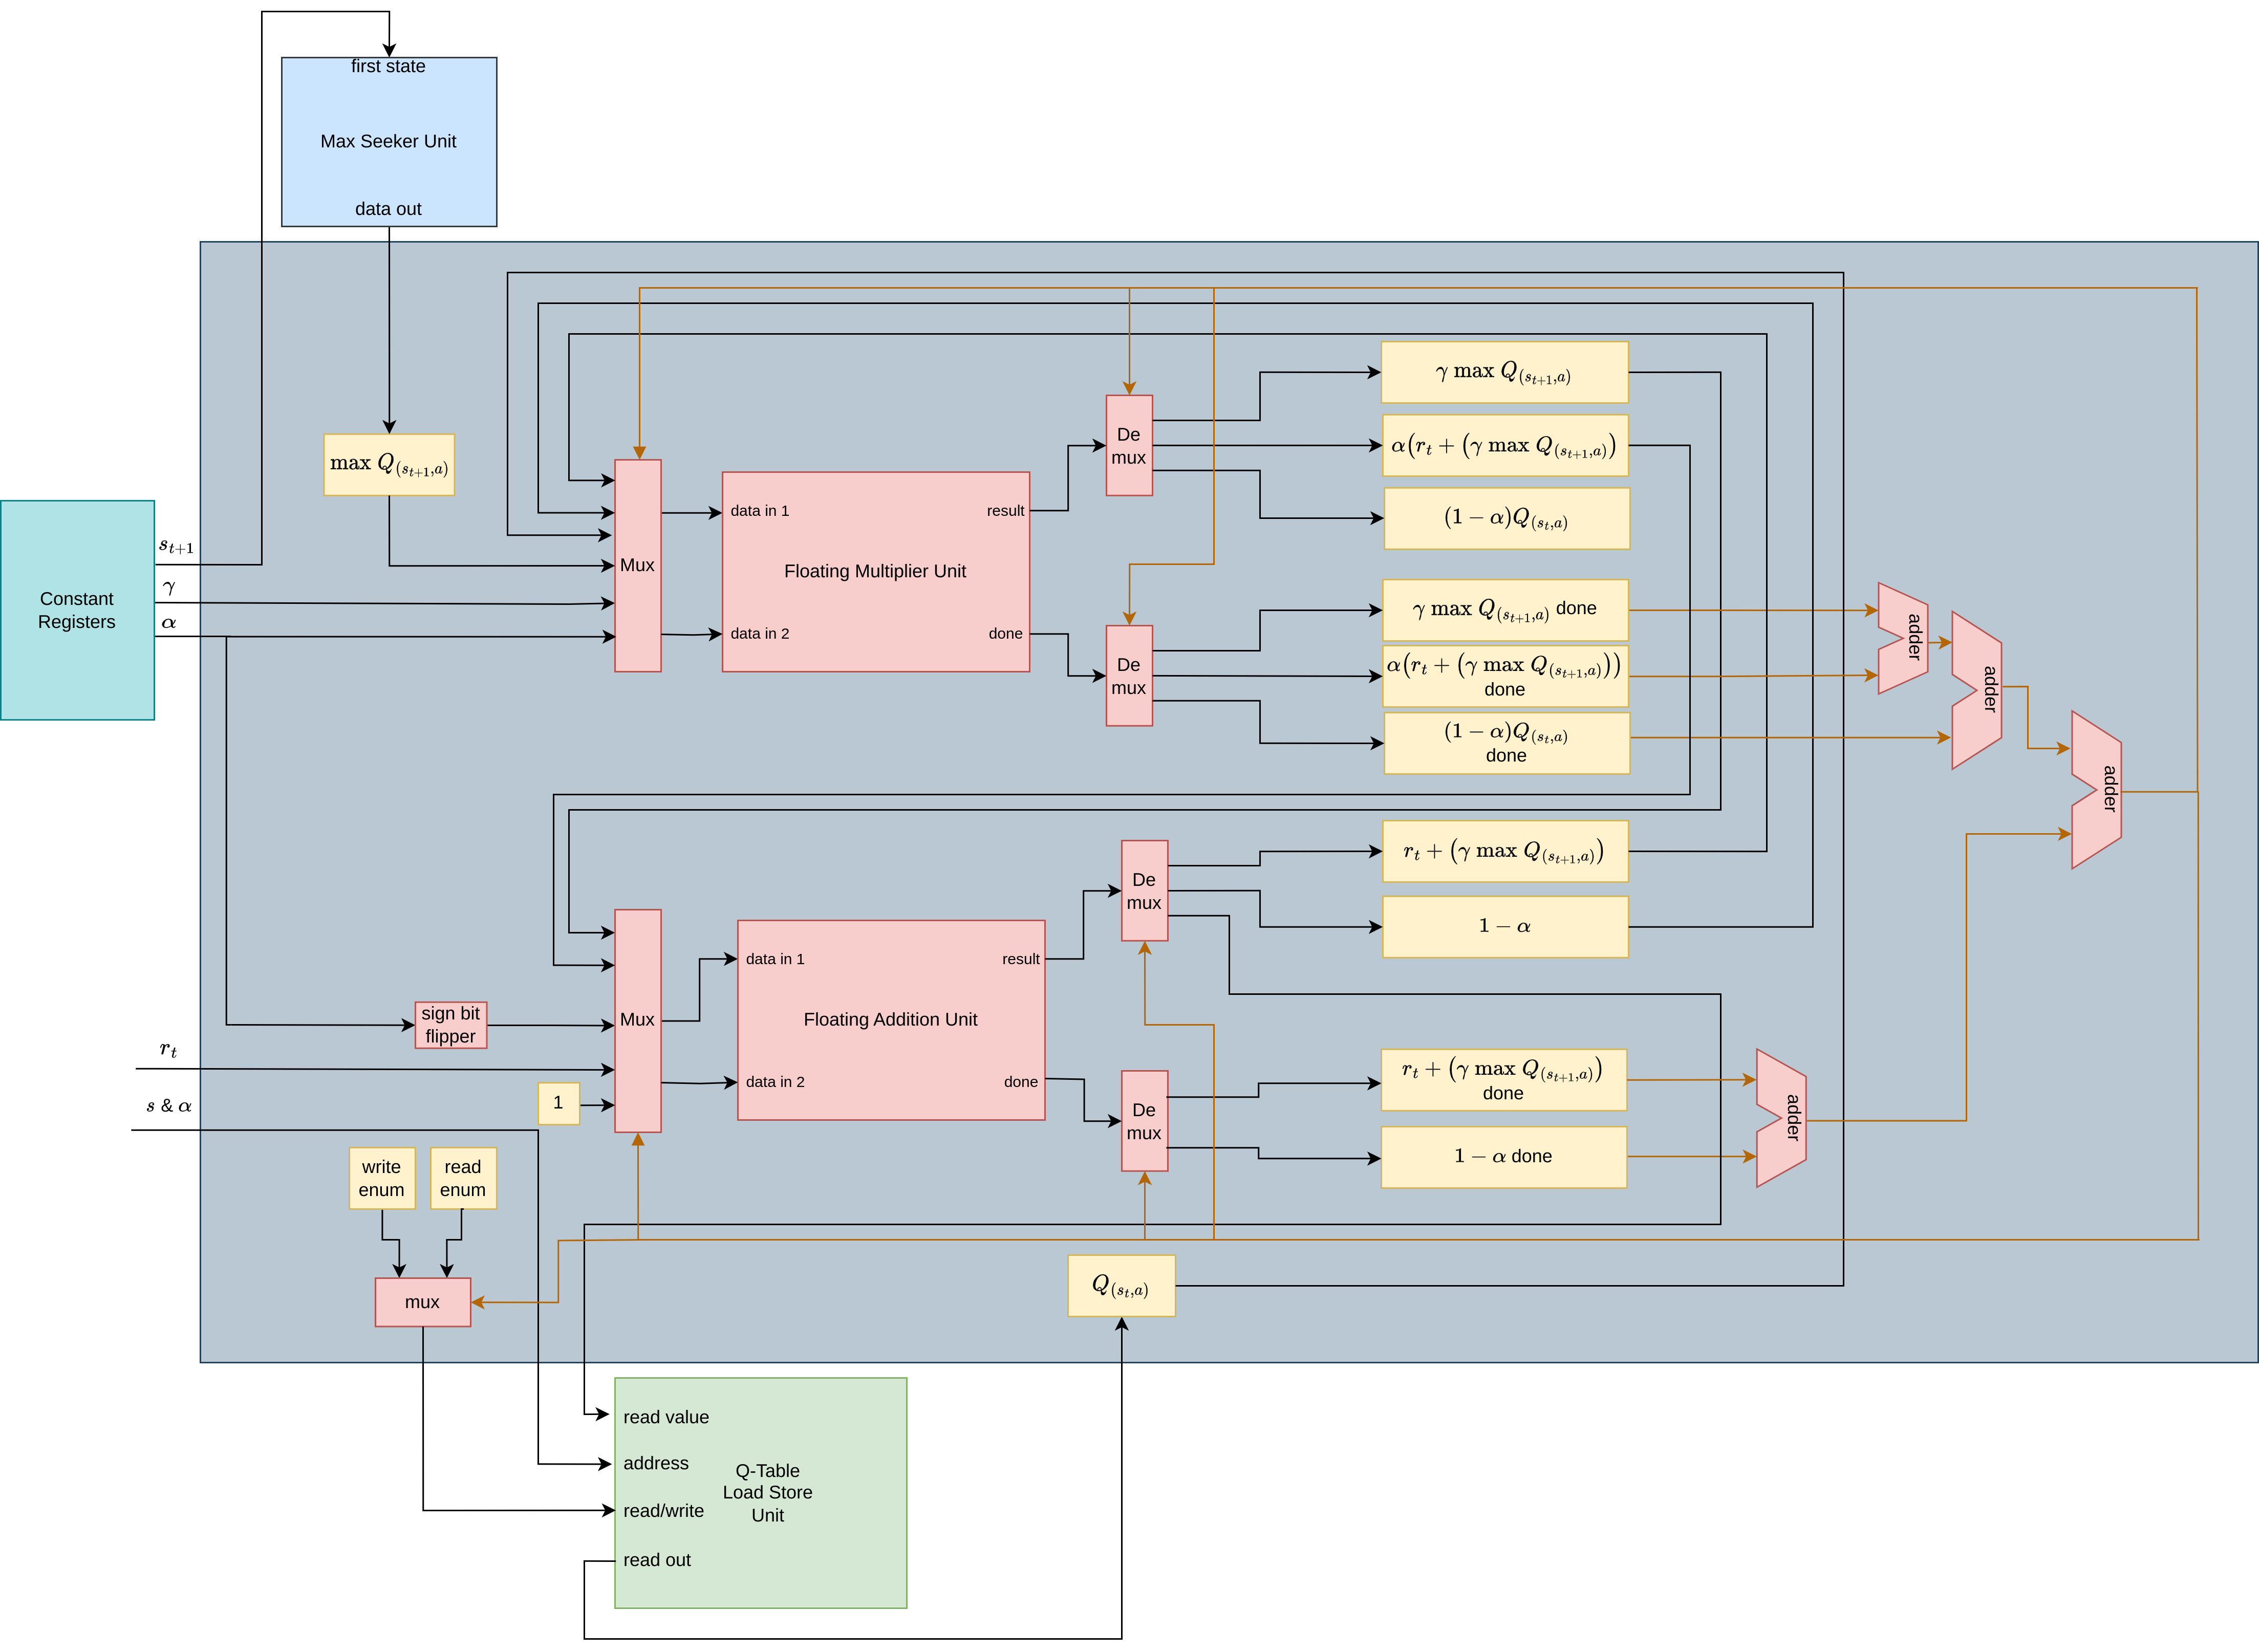
\includegraphics[width=1.2\textwidth]{chapter-3/q-table-updater.png}}
	\caption{Ilustrasi Penggunaan \textit{Q-Table Updater}}
	\label{fig:q-table-updater}
\end{figure}

\textit{Q-Table Updater} merupakan modul akselerator utama yang digunakan untuk menghitung nilai dari Persamaan \ref{eq:q-learning}. Unit ini merupakan unit akselerator yang bekerja asinkron tanpa menunggu seluruh nilai masukannya lengkap. Modul ini memiliki dua modul internal yang berupa \textit{floating addition} dan \textit{multiplier unit}. Kedua modul tersebut digunakan untuk melakukan perhitungan yang diperlukan pada Persamaan \ref{eq:q-learning}. Ketika ada masukan yang sudah siap untuk dihitung maka \textit{Q-Table Updater} akan menghitung nilai dari Persamaan \ref{eq:q-learning} yang dapat dihitung menggunakan informasi yang tersedia. Urutan komputasi persamaan \ref{eq:q-learning} bila seluruh unit menggunakan periode komputasi yang maksimal akan sesuai dengan Gambar \ref{fig:computation-order}.

\begin{figure}[H]
	\centering
	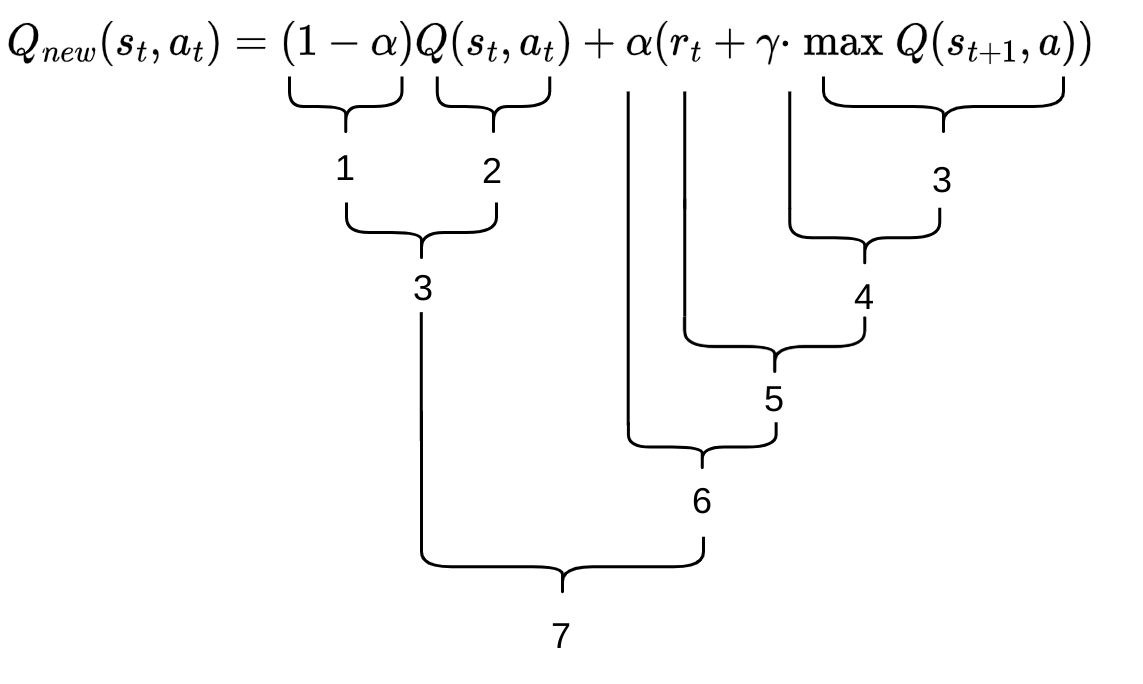
\includegraphics[width=1\textwidth]{chapter-3/computation-order.png}
	\caption{Urutan Komputasi Persamaan \ref{eq:q-learning} pada \textit{Q-Table Updater}}
	\label{fig:computation-order}
\end{figure}

Gambar \ref{fig:computation-order} menggambarkan urutan komputasi yang terjadi apabila masing-masing dari unit yang berhubungan dengan \textit{Q-Table Updater} itu menggunakan periode komputasi yang maksimal. Secara implementasi, urutan periode komputasi maksimal, terkecil menuju terbesar, dari unit yang berhubungan dengan \textit{Q-Table Updater} adalah sebagai berikut.

\begin{enumerate}
	\item \textit{Q-Table \ac{LSU}}: 3 \textit{clock cycles}
	\item \textit{Floating Addition Unit}: 12 \textit{clock cycles}
	\item \textit{Max Seeker Unit}: 13 \textit{clock cycles}
	\item \textit{Floating Multiplying Unit}: 13 \textit{clock cycles}
\end{enumerate}

Dari urutan tersebut dan \textit{hazard management}, maka terbentuklah urutan komputasi yang digambarkan oleh \ref{fig:computation-order}. Selanjutnya, pemakaian dari akselerator perangkat keras yang sudah dijelaskan itu dibuatkan sebuah \ac{BSP} untuk dapat digunakan pada tingkatan perangkat lunak.

\subsection{\ac{BSP} untuk Akses Ekstensi RISC-V pada Perangkat Lunak}

\acf{BSP} merupakan sebuah terminologi di pengembangan sistem tertanam untuk sebuah kumpulan kode yang dibuat untuk menggunakan sebuah fitur tertentu pada sebuah perangkat keras \parencite{xin2021firmware}. Pada kasus di penelitian ini, pembuatan kode untuk mengakses akselerator perangkat keras itu bergantung kepada konvensi biner yang digunakan ekstensi instruksi akselerator dari RISC-V. Gambar \ref{fig:binary-map} merupakan ilustrasi lengkap dari seluruh konvensi biner yang digunakan untuk akselerator perangkat keras pada penelitian ini.

\begin{figure}[H]
	\centering
	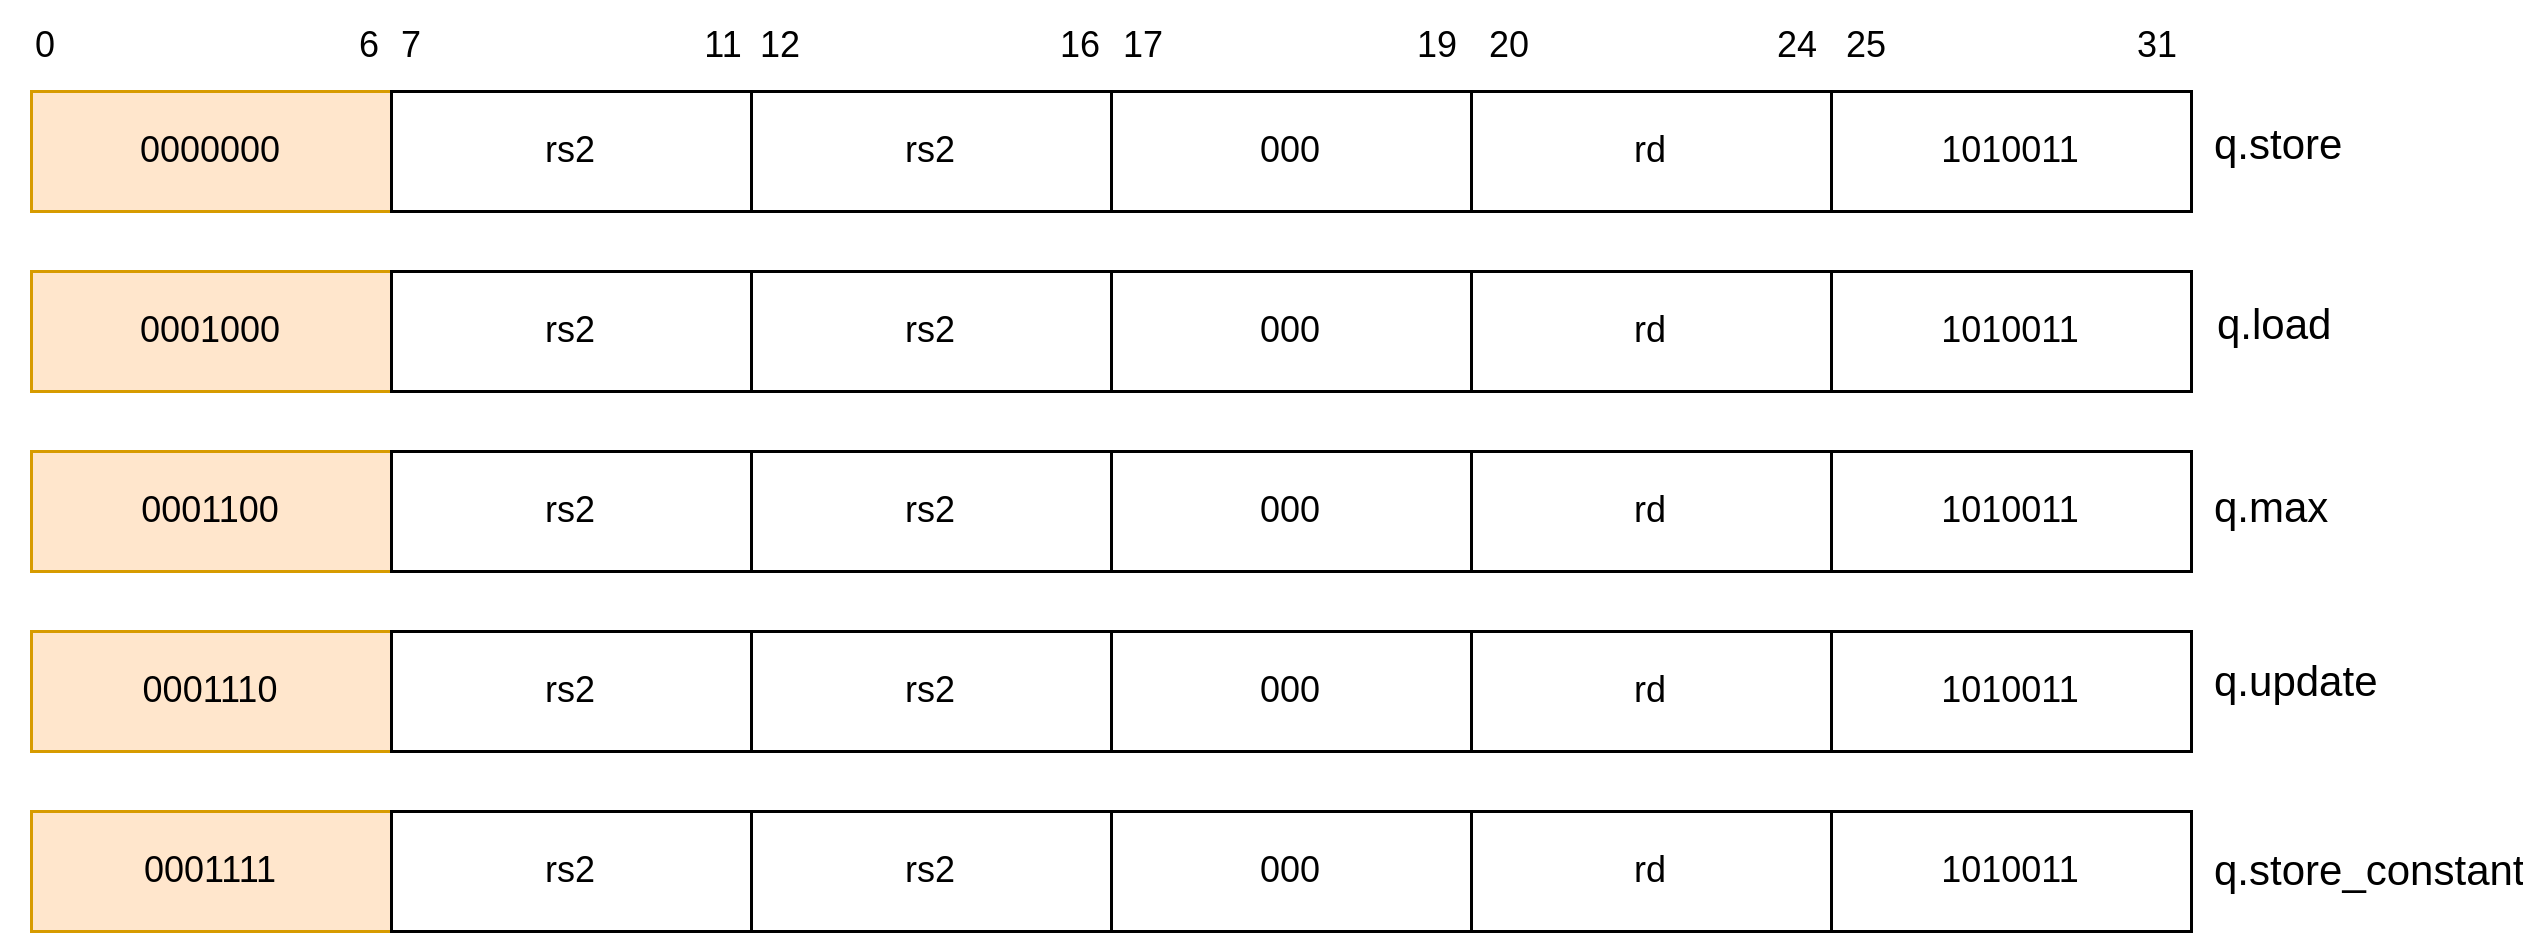
\includegraphics[width=1\textwidth]{chapter-3/binary-map.png}
	\caption{Konvensi Struktur Biner}
	\label{fig:binary-map}
\end{figure}

Konvensi struktur biner yang ada pada Gambar \ref{fig:binary-map} memiliki segmen-segmen yang memiliki fungsi. Dimulai dari kiri secara berurutan, segmen-segmen tersebut adalah funct7, \textit{register source} 1, \textit{register source} 2, funct3, \textit{register destination}, opcode. Funct7, funct3, dan opcode merupakan kombinasi biner yang digunakan untuk dapat mengidentifikasi instruksi yang berbeda. Pada kasus instruksi set ekstensi akselerator ini, funct7 merupakan segmen biner yang digunakan untuk mengidentifikasi secara unik masing-masing instruksi akselerator. Kedua \textit{register source} merupakan \textit{register} yang digunakan untuk memberikan nilai melalui instruksi, sedangkan \textit{register destination} merupakan \textit{register} yang digunakan sebagai tempat disimpannya nilai hasil dari instruksi.

Pada kode bahasa C, contoh pembuatan \ac{BSP} dilakukan seperti pada Gambar \ref{fig:bsp-example}.

\begin{figure}[H]
	\centering
	\begin{lstlisting}[language=C,escapechar=|,numbers=left]
float storeQValue(float rs1, unsigned int rs2) {
	float result;
	asm("lw t3, %0;" : "=m"(rs1));
	asm("lw t4, %0;" : "=m"(rs2));
	asm(".word 0x01ce8f53;"); |\label{algline:assembly-binary}|
	asm("sw t5, %0;" : "=m"(result)); 
	return result;
}
\end{lstlisting}
	\caption{Contoh Fungsi \ac{BSP}}
	\label{fig:bsp-example}
\end{figure}

Penulisan fungsi untuk \ac{BSP} seperti contoh Gambar \ref{fig:bsp-example} memerlukan pemilihan tiga \textit{register} dari RISC-V yang dapat digunakan sebagai \textit{register} temporer. Lalu, ketiga \textit{register} temporer tersebut digunakan untuk \textit{register source} 1, \textit{register source} 2, dan \textit{register destination}. Terakhir, alamat-alamat dari \textit{register} tersebut digunakan untuk membuat instruksi assembly dengan konvensi biner pada Gambar \ref{fig:binary-map}.

Pada tahapan awal, pemilihan \textit{register} temporer dapat mengacu kepada Gambar \ref{fig:riscv-registers} yang merupakan daftar resmi \textit{register} RISC-V beserta kegunaannya.

\begin{figure}[H]
	\centering
	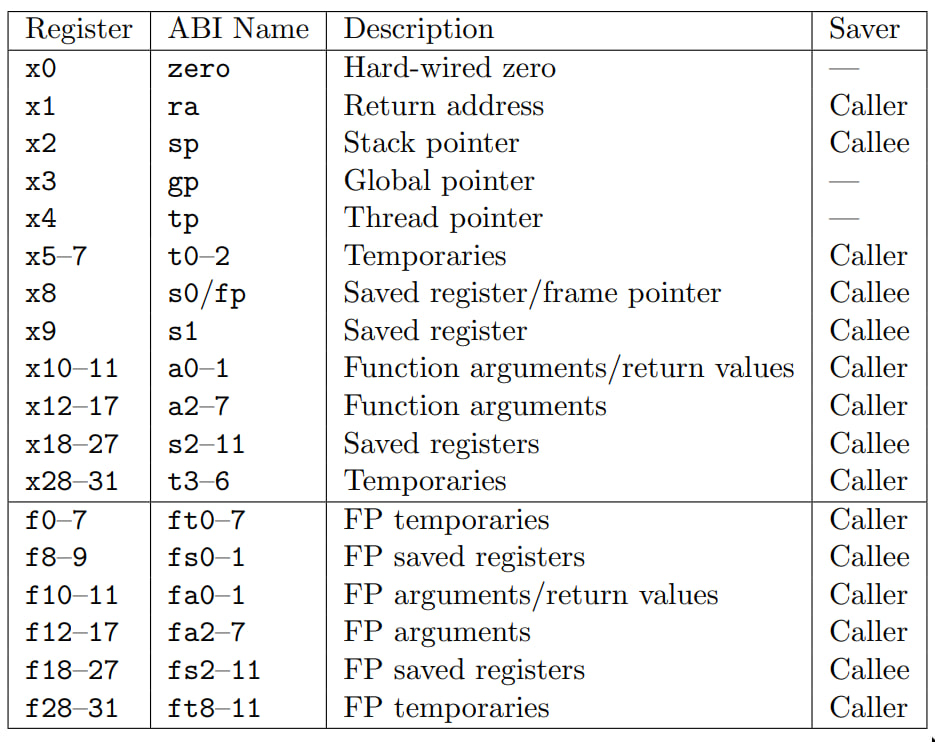
\includegraphics[width=0.8\textwidth]{chapter-3/riscv-registers.jpg}
	\caption{Daftar \textit{Register} RISC-V}
	\label{fig:riscv-registers}
\end{figure}

Pada Gambar \ref{fig:riscv-registers}, terdapat tujuh \textit{register} yang dapat digunakan sebagai \textit{register} temporer yaitu t0 hingga t6. Masing-masing \textit{register} ini, memiliki alamat asli yang terletak pada \ac{RAM} dari \textit{processor}. Alamat tersebut, ditandai oleh kolom \textit{Register} pada Gambar \ref{fig:riscv-registers}. Contohnya, pada Gambar \ref{fig:bsp-example}, \ac{BSP} yang dibangun merupakan \ac{BSP} untuk instruksi q.store dengan t3 dan t4 untuk \textit{register} source dan t5 untuk \textit{register destination}. Hasil instruksi dalam bentuk heksadesimal yang dibangun pada Gambar \ref{fig:bsp-example} baris \ref{algline:assembly-binary} adalah 0x01ce8f53 atau 00000001110011101000111101010011 pada representasi binernya. Secara detail, berikut merupakan penjelasan dari segmen-segmen yang ada pada Gambar \ref{fig:binary-map}.

\begin{enumerate}
	\item funct7: 0000000
	\item \textit{register source} 1: 11100
	\item \textit{register source} 2: 11101
	\item funct3: 000
	\item \textit{register destination}: 11110
	\item opcode: 1010011
\end{enumerate}

\subsection{Pengujian Akurasi Akselerator Menggunakan \textit{Verilator}}
\label{subsec:verilator}

Pengujian akurasi akselerator, dilakukan menggunakan \textit{verilator}. \textit{Verilator} \parencite{verilator2024github} merupakan aplikasi perangkat lunak yang dapat menghasilkan uji sintesis yang berupa \textit{timing diagram} untuk melihat apakah hasil implementasi akselerator perangkat keras sudah sesuai dengan hasil kode dari perangkat lunak. Pada penelitian ini, \textit{verilator} akan digunakan untuk mensintesis sebuah program dengan bahasa C menjadi \textit{timing diagram} dari \textit{register-register} verilog pada VeeR EL2. \textit{Timing diagram} tersebut, akan digunakan untuk mengecek kesesuaian hasil dari implementasi perangkat lunak dengan implementasi pada akselerator.
